\chapter{线性算子半群}\vspace{-2em}

\section{Banach空间中的常微分方程}

具Lipschitz连续右端项的常微分方程的经典存在唯一性理论，可不作实质性改动地推广至Banach空间.设 $X$ 是Banach空间， $F : X \mapsto  X$ 是Lipschitz连续映射，即满足
\begin{equation}\tag{7.1}\label{eq:lipschitz-F}
\| F\left( x\right)  - F\left( y\right) \|  \leq  L\| x - y\|
\end{equation}

对某个Lipschitz常数 $L$ 及所有 $x,y \in  X$ .

给定初始点 $\bar{x} \in  X$ ，考虑Cauchy问题
\begin{equation}\tag{7.2}\label{eq:cauchy-problem-ode}
\dot{x}\left( t\right)  = F\left( {x\left( t\right) }\right) ,\;x\left( 0\right)  = \bar{x}.
\end{equation}

此处及后续章节中，上点号表示对时间的导数.与有限维情形类似，可利用压缩映射定理证明解的整体存在性与唯一性.
\begin{theorem}[Lipschitz连续右端项常微分方程Cauchy问题解的存在唯一性]\label{thm:lipschitz-ode-existence-uniqueness}
设 $X$ 为 Banach 空间，且向量场 $F : X \mapsto  X$ 满足 Lipschitz 条件\eqref{eq:lipschitz-F}.则对任意 $\bar{x} \in  X$ ，Cauchy 问题\eqref{eq:cauchy-problem-ode} 存在唯一解 $t \mapsto  x\left( t\right)$ ，定义于所有 $t \in  \mathbb{R}$ 上.
\end{theorem}

\begin{proof}
任取 $T > 0$ ，考虑所有连续映射 $w : \left(  {0,T}\right)   \mapsto  X$ 构成的 Banach 空间 $\mathcal{C}\left( {\left(  {0,T}\right)  ;X}\right)$，其配备等价范数
\begin{equation}\tag{7.3}\label{eq:equiv-norm-dagger}
\|w\|_{\dagger} \doteq  \mathop{\max }\limits_{{t \in  \left(  {0,T}\right)  }}{e}^{-{2Lt}}\| w\left( t\right) \| .
\end{equation}

注意:函数 $x : \left(  {0,T}\right)   \mapsto  X$ 是 Cauchy 问题\eqref{eq:cauchy-problem-ode} 的解，当且仅当 $x\left( \cdot \right)$ 是 Picard 算子的不动点
\begin{equation}\tag{7.4}\label{eq:picard-operator}
\Phi \left( w\right) \left( t\right)  \doteq  \bar{x} + {\int }_{0}^{t}F\left( {w\left( s\right) }\right) {\d s},\;t \in  \left(  {0,T}\right)  .
\end{equation}

我们断言: $\Phi$ 关于等价范数\eqref{eq:equiv-norm-dagger} 是严格压缩映射.事实上，对任意 $u,v \in  \mathcal{C}\left( {\left(  {0,T}\right)  ;X}\right)$，令 $\delta  \doteq  \|u - v\|_{\dagger}$ .由定义\eqref{eq:equiv-norm-dagger}，这蕴含
\[
\| u\left( s\right)  - v\left( s\right) \|  \leq  \delta {e}^{2Ls}\;\forall\,s \in  \left(  {0,T}\right)  .
\]

对每个 $t \in  \left(  {0,T}\right)$ ，由 Lipschitz 连续性假设\eqref{eq:lipschitz-F} 可得
{\begin{align*}
    &{e}^{-{2Lt}}\norm{\Phi \left( u\right) \left( t\right)  - \Phi \left( v\right) \left( t\right) } = {e}^{-{2Lt}}\norm{{\int }_{0}^{t}\left( {F\left( {u\left( s\right) }\right)  - F\left( {v\left( s\right) }\right) }\right) {\d s}}\\
    &\quad \leq  {e}^{-{2Lt}}{\int }_{0}^{t}\norm{F\left( {u\left( s\right) }\right)  - F\left( {v\left( s\right) }\right) }{\d s} \leq  {e}^{-{2Lt}}{\int }_{0}^{t}L\| u\left( s\right)  - v\left( s\right) \| {\d s}\\
    &\quad\leq  {e}^{-{2Lt}}{\int }_{0}^{t}{L\delta }{e}^{2Ls}{\d s} < \frac{\delta }{2}.
\end{align*}}


因此
\begin{equation}\tag{7.5}\label{eq:picard-contraction}
\|\Phi \left( u\right)  - \Phi \left( v\right) \|_{\dagger} \leq  \frac{1}{2}\|u - v\|_{\dagger}.
\end{equation}

现应用压缩映射定理，得到 $\Phi$ 的唯一不动点，即存在唯一的连续映射 $x\left( \cdot \right)$ ，使得
\[
x\left( t\right)  = \bar{x} + {\int }_{0}^{t}F\left( {x\left( s\right) }\right) {\d s}\;\forall\,t \in  \left(  {0,T}\right)  .
\]

该函数 $x\left( \cdot \right)$ 即为 Cauchy 问题的唯一解.通过时间反演，可在任意形如 $\left(  {-T,0}\right)$ 的时间区间上构造唯一解.
\end{proof}

图\ref{fig:euler-approximation}展示了构造 Cauchy 问题\eqref{eq:cauchy-problem-ode} 近似解的两种经典方法.以下固定时间步长 $h > 0$ ，并定义时刻 ${t}_{j} = j \cdot  h,j = 0,1,2,\ldots$

\begin{figure}[htbp]
\centering
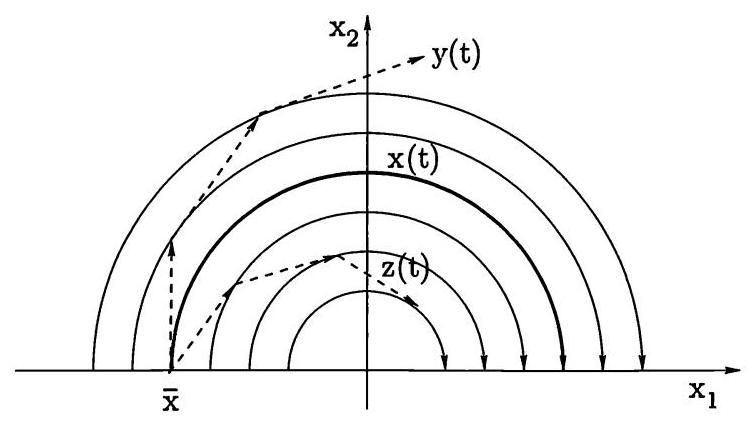
\includegraphics[width=0.7\textwidth]{images/bo_d6ik6nn7aajc739ct1l0_129_334_235_748_423_0.jpg}
\caption{系统 ${\dot{x}}_{1} = {x}_{2},{\dot{x}}_{2} = \; - {x}_{1}$ 的 Euler 近似.其中 $x\left( \cdot \right)$ 为精确解， $y\left( \cdot \right)$ 是由前向 Euler 格式得到的分段仿射近似，而 $z\left( \cdot \right)$ 是由后向 Euler 格式得到.}
\label{fig:euler-approximation}
\end{figure}

— 前向 Euler 近似:近似解在时刻 ${t}_{j}$ 的取值按如下公式归纳定义
\begin{equation}\tag{7.6}\label{eq:forward-euler}
x\left( {t}_{j + 1}\right)  = x\left( {t}_{j}\right)  + {hF}\left( {x\left( {t}_{j}\right) }\right) .
\end{equation}

— 后向 Euler 近似:近似解在时刻 ${t}_{j}$ 的取值由下式确定
\begin{equation}\tag{7.7}\label{eq:backward-euler}
x\left( {t}_{j + 1}\right)  = x\left( {t}_{j}\right)  + {hF}\left( {x\left( {t}_{j + 1}\right) }\right) .
\end{equation}

两种情形下，一旦在离散时刻集 ${t}_{j}$ 上计算出 $x\left( {t}_{j}\right)$ 的值，即可将近似解延拓至所有实数 $t \geq  0$ ，令 $t \mapsto  x\left( t\right)$ 在每个区间 $\left(  {{t}_{j - 1},{t}_{j}}\right)$ 上为仿射函数.

前向 Euler 近似易于构造:在整个时间区间 $\left(  {{t}_{j},{t}_{j + 1}}\right)$ 上，令导数 $\dot{x}\left( t\right)$ 保持恒定，且等于初值点处 $F$ 的取值:
\[
\dot{x}\left( t\right)  = F\left( {x\left( {t}_{j}\right) }\right) ,\;t \in  \left(  {{t}_{j},{t}_{j + 1}}\right)  .
\]

另一方面，在后向Euler近似中，对于 $t \in  \left(  {{t}_{j},{t}_{j + 1}}\right)$ ，我们令导数 $\dot{x}\left( t\right)$ 保持恒定，且等于 $F$ 在终点处的值:
\[
\dot{x}\left( t\right)  = F\left( {x\left( {t}_{j + 1}\right) }\right) ,\;t \in  \left(  {{t}_{j},{t}_{j + 1}}\right)  .
\]

此时，给定 $x\left( {t}_{j}\right)$ ，为求得 $x\left( {t}_{j + 1}\right)$ ，需求解隐式方程\eqref{eq:backward-euler}.因此，后向Euler近似需要更多的计算工作量；但另一方面，其通常具有更优的稳定性和收敛性.

\subsection{线性齐次常微分方程}

设 $A : {\mathbb{R}}^{n} \mapsto  {\mathbb{R}}^{n}$ 为一线性算子.则线性Cauchy问题的解
\begin{equation}\tag{7.8}\label{eq:linear-ode}
\dot{x} = {Ax},\;x\left( 0\right)  = \bar{x}
\end{equation}

是映射 $t \mapsto  {e}^{tA}\bar{x}$ ，其中
\begin{equation}\tag{7.9}\label{eq:exp-series}
{e}^{tA} \doteq  \mathop{\sum }\limits_{{k = 0}}^{\infty }\frac{{t}^{k}{A}^{k}}{k!}
\end{equation}

该公式对任意Banach空间 $X$ 上的有界线性算子 $A$ 依然成立.我们注意到，\eqref{eq:exp-series}式中的级数对每个 $t \in  \mathbb{R}$ 均绝对收敛.此外，指数映射具有如下性质:

(i) ${e}^{0A} = I$ ，即恒等映射.

(ii) ${e}^{sA}{e}^{tA} = {e}^{\left( {s + t}\right) A}$ (半群性质).

(iii) 对每个 $\bar{x} \in  X$ ，映射 $t \mapsto  {e}^{tA}\bar{x}$ 连续.

由 (i)-(ii) 可知，算子族 $\left\{  {{e}^{tA};t \geq  0}\right\}$ 构成一个线性算子群.

更一般地，线性半群理论研究线性算子与其指数之间的对应关系.
\[
A \leftrightarrow  \left\{  {{e}^{tA};t \geq  0}\right\}
\]

当 $A$ 为有界线性算子时，其指数函数由收敛级数\eqref{eq:exp-series}给出.反之，给定算子族 ${e}^{tA}$，可通过极限恢复 $A$
\[
A = \mathop{\lim }\limits_{{t \rightarrow  0 + }}\frac{{e}^{tA} - I}{t}.
\]

存在重要情形:对每个 $t \geq  0$ ，算子 ${e}^{tA}$ 均有界，而 $A$ 却是无界算子.这恰是半群理论最具意义的应用，广泛用于抛物型或双曲型偏微分方程的分析.

\begin{instance}\label{ins:diagonal-matrix-exponential}
若 $A : {\mathbb{R}}^{n} \mapsto  {\mathbb{R}}^{n}$ 为一对角矩阵，则其指数可直接计算.事实上
\[
A = \left( \begin{matrix} {\lambda }_{1} & & 0 \\  \vdots & & \vdots \\  0 & & {\lambda }_{n} \end{matrix}\right) ,\;{e}^{tA} = \left( \begin{matrix} {e}^{t{\lambda }_{1}} & & 0 \\  \vdots & & \vdots \\  0 & & {e}^{t{\lambda }_{n}} \end{matrix}\right) .
\]

注意，对应的算子范数为
\[
\| A\| \; = \;\mathop{\max }\limits_{k}\;\left| {\lambda }_{k}\right| ,\;\| {e}^{tA}\| \; = \;\mathop{\max }\limits_{k}\left| {e}^{t{\lambda }_{k}}\right| .
\]
\end{instance}

\begin{instance}\label{ins:diagonal-operator-l1}
设 ${\ell }^{1}$ 为赋范为 $x = \left( {{x}_{1},{x}_{2},{x}_{3},\ldots }\right)$ 的复数序列全体构成的Banach空间
\[
\| x{\| }_{{\ell }^{1}} \doteq  \mathop{\sum }\limits_{k}\left| {x}_{k}\right|
\]

对任意复数序列 ${\left( {\lambda }_{k}\right) }_{k \geq  1}$ ，考虑线性算子
\begin{equation}\tag{7.10}\label{eq:diagonal-operator-l1}
{Ax} \doteq  \left( {{\lambda }_{1}{x}_{1},{\lambda }_{2}{x}_{2},{\lambda }_{3}{x}_{3},\ldots }\right) .
\end{equation}

相应的指数算子为
\[
{e}^{tA}x = \left( {{e}^{t{\lambda }_{1}}{x}_{1},{e}^{t{\lambda }_{2}}{x}_{2},{e}^{t{\lambda }_{3}}{x}_{3},\ldots }\right) .
\]

需注意，该量
\[
\| A\|  = \mathop{\sup }\limits_{k}\left| {\lambda }_{k}\right|
\]
可能为无穷大，但与此同时，范数
\[
\norm{e}^{tA} = \mathop{\sup }\limits_{k}\left| {e}^{t{\lambda }_{k}}\right|
\]
对每个 $t \geq  0$ 均可有界.事实上，如图\ref{fig:spectrum-regions}所示，假设所有特征值 ${\lambda }_{k}$ 的实部一致上有界，即
\[
{\lambda }_{k} = {\alpha }_{k} + i{\beta }_{k},\;{\alpha }_{k} \leq  \omega \;\forall\,k \geq  1,
\]

对某个常数 $\omega  \in  \mathbb{R}$ 成立.则
\begin{equation}\tag{7.11}\label{eq:exp-bound-semigroup}
\left| {e}^{t{\lambda }_{k}}\right|  = \left| {e}^{t{\alpha }_{k}}\right|  \leq  {e}^{t\omega }\;\forall\,t \geq  0.
\end{equation}

因此，对每个 $t \geq  0$ ，算子 ${e}^{tA}$ 均有界，即 $\norm{e}^{tA} \leq  {e}^{t\omega }$ .

另两种情形亦值得探讨.

情形1:假设所有特征值 ${\lambda }_{k}$ 的实部既有上界也有下界，即
\[
- \omega  \leq  {\alpha }_{k} \leq  \omega
\]

对某个常数 $\omega  > 0$ 及所有 $k \geq  1$ 成立.则对所有 $t \in  \mathbb{R}$ ，有估计式
\begin{equation}\tag{7.12}\label{eq:exp-bound-group}
\left| {e}^{t{\lambda }_{k}}\right|  = \left| {e}^{t{\alpha }_{k}}\right|  \leq  {e}^{\left| t\right| \omega }
\end{equation}

故算子 ${e}^{tA}$ 对所有 $t < 0$ 均有界.这表明微分方程\eqref{eq:linear-ode}既可正向也可反向求解.算子族 $\left\{  {{e}^{tA};t \in  \mathbb{R}}\right\}$ 构成一族有界线性算子群.

情形2:假设所有特征值 ${\lambda }_{k} = {\alpha }_{k} + i{\beta }_{k}$ 均位于复平面的一个扇形区域内.更准确地说，假设存在 $\omega  \in  \mathbb{R}$ 与角度 $0 < \overline{\theta } < \pi /2$ ，使得对每个 $k$ ，可写为
\begin{equation}\tag{7.13}\label{eq:sectorial-eigs}
{\alpha }_{k} = \omega  - {r}_{k}\cos {\theta }_{k},\;{\beta }_{k} =  - {r}_{k}\sin {\theta }_{k}
\end{equation}

其中 ${r}_{k} \geq  0$ 与 ${\theta }_{k} \in  \left(  {-\overline{\theta },\overline{\theta }}\right)$ 为某常数.

此时，由于 ${\alpha }_{k} \leq  \omega$ ，显然\eqref{eq:exp-bound-semigroup}成立，且算子 $\norm{e}^{tA}$ 对每个 $t \geq  0$ 均有界.然而，更强的结论成立:对每个 $t > 0$ ，复合算子 $A{e}^{tA}$ 均有界.事实上
{\begin{align*}
    \norm{A{e}^{tA}} &= \mathop{\sup }\limits_{k}\left| {{\lambda }_{k}{e}^{t{\lambda }_{k}}}\right|  \leq  \mathop{\sup }\limits_{k}\left( {\omega  + {r}_{k}}\right) {e}^{\left( {\omega  - {r}_{k}\cos {\theta }_{k}}\right) t}\\
    &\leq  \mathop{\sup }\limits_{{r \geq  0,\left| \theta \right|  \leq  \overline{\theta }}}\left( {\omega  + r}\right) {e}^{\left( {\omega  - r\cos \theta }\right) t} \leq  \mathop{\sup }\limits_{{r \geq  0}}\left( {\omega  + r}\right) {e}^{\left( {\omega  - r\cos \overline{\theta }}\right) t} <  + \infty ,
\end{align*}}

因为 $\cos \overline{\theta } > 0$ .此时， $A$ 称为扇形算子.

即使初始数据 $\bar{x}$ 不在算子 $A$ 的定义域内，对每个 $t > 0$ ，仍有 $x\left( t\right)  = {e}^{tA}\bar{x} \in  \operatorname{Dom}\left( A\right)$ .

\begin{figure}[htbp]
\centering
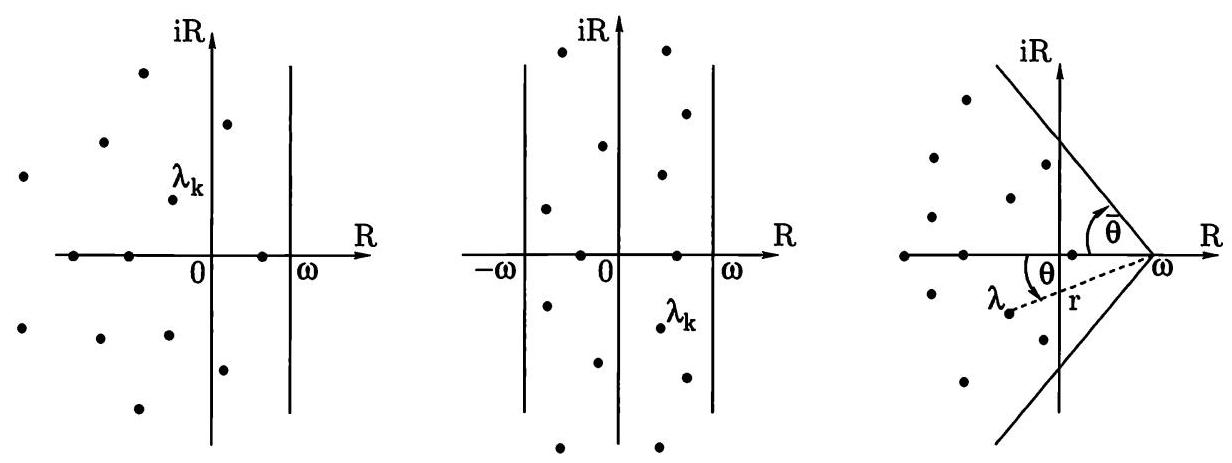
\includegraphics[width=1.0\textwidth]{images/bo_d6ik6nn7aajc739ct1l0_132_122_1026_1232_463_0.jpg}
\caption{左:当算子 $A$ (见\eqref{eq:diagonal-operator-l1}式)的所有特征值 ${\lambda }_{k}$ 的实部满足 $\operatorname{Re}\left( {\lambda }_{k}\right)  \leq  \omega$ 时，则对每个 $t \geq  0$ ，指数算子均有界: $\norm{e}^{tA} \leq  {e}^{t\omega }$ .中:若所有特征值 ${\lambda }_{k}$ 满足 $\operatorname{Re}\left( {\lambda }_{k}\right)  \in  \left(  {-\omega ,\omega }\right)$ ，则对每个 $t \in  \mathbb{R}$ ，指数算子均有界: $\norm{e}^{tA} \leq  {e}^{\left| t\right| \omega }$ .右:若所有特征值 ${\lambda }_{k}$ 位于复平面中一个张角为 $\overline{\theta } < \pi /2$ 的扇形内，则对每个 $t > 0$ ，算子 $A{e}^{tA}$ 同样有界.}
\label{fig:spectrum-regions}
\end{figure}
\end{instance}

\section{线性算子半群}

考虑Banach空间 $X$ 中的线性演化方程，例如
\begin{equation}\tag{7.14}\label{eq:evolution-equation}
\frac{\d}{\d t}u\left( t\right)  = {Au}\left( t\right) ,\;u\left( 0\right)  = \bar{u} \in  X.
\end{equation}

当$t \geq  0$ ，我们希望将解表示为$u\left( t\right)  = {e}^{tA}\bar{u}$ ，其中 $\left\{  {{e}^{tA};t \geq  0}\right\}$ 是一族线性算子.

\begin{instance}\label{ins:transport-equation}
考虑偏微分方程 ${u}_{t} - {u}_{x} = 0$ .该方程可重写为形式\eqref{eq:evolution-equation}，其中 $A = \frac{\partial }{\partial x}$ 是一个微分算子.作为函数空间，可取 $X = {L}^{p}\left( \mathbb{R}\right)$ ，其中 $p \in (1,\infty)$ 为某常数.显然，微分算子 $A$ 是无界的，其定义域为所有绝对连续函数 $u \in  {L}^{p}\left( \mathbb{R}\right)$ ，且其导数 ${u}_{x} \in  {L}^{p}\left( \mathbb{R}\right)$ 满足相应条件.另一方面，对任意初值 $\bar{u} \in  {L}^{p}$ ，初值问题的解
\[
{u}_{t} = {u}_{x},\;u\left( {0,x}\right)  = \bar{u}\left( x\right)
\]

可显式计算:
\[
u\left( {t,x}\right)  = \bar{u}\left( {x + t}\right) ,\;t \in  \mathbb{R}.
\]

这表明，尽管微分算子 $A = \frac{\partial }{\partial x}$ 是无界的，相应的指数算子 ${e}^{tA}$ 却是一致有界的:
\[
\left( {{e}^{tA}\bar{u}}\right) \left( x\right)  = \bar{u}\left( {x + t}\right)
\]
从而对每个 $t \in  \mathbb{R}$ 均有 $\norm{e}^{tA} = 1$ .
\end{instance}

在线性半群理论中，需考虑两个基本问题:

\begin{enumerate}[(1)]
    \item 给定一族线性算子半群 $\left\{  {{S}_{t};t \geq  0}\right\}$ ，求其生成元，即求算子$A$ ，使得${S}_{t} = {e}^{tA}$.
    \item 给定一线性算子 $A$ ，判断它是否生成一个半群 $\left\{  {{e}^{tA};t \geq  0}\right\}$ ，并研究其性质.
\end{enumerate}

在应用中，(2)显然更为重要；然而，为推进理论发展，从(1)入手则更为方便.

\subsection{半群的定义与基本性质}

\begin{definition}[强连续线性算子半群]\label{def:C0-semigroup}
设 $X$ 为一Banach空间. $X$ 上的\colorbf{强连续线性算子半群}是指一族线性映射 $\left\{  {{S}_{t};t \geq  0}\right\}$，满足如下性质.
\begin{enumerate}[(i)]
    \item 每个 ${S}_{t} : X \mapsto  X$ 均为有界线性算子.
    \item 对任意 $s,t \geq  0$ ，复合运算满足 ${S}_{t}{S}_{s} = {S}_{t + s}$；且 ${S}_{0} = I$.
    \item 对任意 $u \in  X$ ，映射 $t \mapsto  {S}_{t}u$ 是从 $(0,\infty )$ 到 $X$ 的连续映射.
\end{enumerate}
\end{definition}
\begin{definition}[$\omega$类算子半群]\label{def:semigroup-type}
    若强连续线性算子半群满足如下估计式：
    \begin{equation}\tag{7.15}\label{eq:semigroup-type}
\norm{S}_{t} \leq  {e}^{t\omega }\;\forall\,t \geq  0.
\end{equation}
    则称 $\left\{  {{S}_{t};t \geq  0}\right\}$ 为\colorbf{$\omega$类算子半群}.\par
    特别地，当$\omega = 0$时，称$\left\{{{S}_{t};t \geq  0}\right\}$为\colorbf{压缩算子半群}.
\end{definition}
事实上，对压缩算子半群，对于每个 $t \geq  0$ 均有 $\norm{S}_{t} \leq  1$ ，故
\[
\norm{{S}_{t}u - {S}_{t}v} \leq  \| u - v\| \;\forall\,\;u,v \in  X,t \geq  0.
\]
\begin{definition}[算子半群的生成元]
    线性算子
\begin{equation}\tag{7.16}\label{eq:generator-def}
{Au} \doteq  \mathop{\lim }\limits_{{t \rightarrow  0 + }}\frac{{S}_{t}u - u}{t}
\end{equation}
称为半群 $\left\{  {{S}_{t};t \geq  0}\right\}$ 的\colorbf{生成元}.其定义域 $\operatorname{Dom}\left( A\right)$ 是使\eqref{eq:generator-def}中极限存在的所有 $u \in  X$ 构成的集合.
\end{definition}



对给定的 $\bar{u} \in  X$ ，我们将映射 $t \mapsto  {S}_{t}\bar{u}$ 视为线性常微分方程\eqref{eq:evolution-equation}的解.注意，此处在某种意义上我们是逆向处理该问题:给定解 $u\left( t\right)  = {S}_{t}\bar{u}$ ，我们试图重构演化方程，并找出算子 $A$ .接下来推导半群 $S$ 及其生成元 $A$ 的若干基本性质.


\begin{theorem}[半群的性质]\label{thm:semigroup-properties}
设 $\left\{  {{S}_{t};t \geq  0}\right\}$ 是强连续半群， $A$ 为其生成元，且假设 $\bar{u} \in  \operatorname{Dom}\left( A\right)$ .则
\begin{enumerate}[(i)]
    \item 对每个 $t \geq  0$ ，均有 ${S}_{t}\bar{u} \in  \operatorname{Dom}\left( A\right)$ 且 $A{S}_{t}\bar{u} = {S}_{t}A\bar{u}$.
    \item 映射 $t \mapsto  u\left( t\right)  \doteq  {S}_{t}\bar{u}$ 连续可微，且为初值问题\eqref{eq:evolution-equation}的解.
\end{enumerate}
\end{theorem}

\begin{proof}
1. 设 $\bar{u} \in  \operatorname{Dom}\left( A\right)$ ，即\eqref{eq:generator-def}中的极限存在.则
\[
\mathop{\lim }\limits_{{s \rightarrow  0 + }}\frac{{S}_{s}{S}_{t}\bar{u} - {S}_{t}\bar{u}}{s} = \mathop{\lim }\limits_{{s \rightarrow  0 + }}\frac{{S}_{t}{S}_{s}\bar{u} - {S}_{t}\bar{u}}{s} = {S}_{t}\mathop{\lim }\limits_{{s \rightarrow  0 + }}\frac{{S}_{s}\bar{u} - \bar{u}}{s} = {S}_{t}A\bar{u}.
\]

因此 ${S}_{t}\bar{u} \in  \operatorname{Dom}\left( A\right)$ 且 $A{S}_{t}\bar{u} = {S}_{t}A\bar{u}$ ，从而证得(i).

\noindent 2. 接着，设 $\bar{u} \in  \operatorname{Dom}\left( A\right) ,t > 0$ .由半群性质可得
\begin{gather*}
\mathop{\lim }\limits_{{h \rightarrow  0 + }}\left\{  {\frac{{S}_{t}\bar{u} - {S}_{t - h}\bar{u}}{h} - {S}_{t}A\bar{u}}\right\}   = \mathop{\lim }\limits_{{h \rightarrow  0 + }}\left\{  {{S}_{t - h}\left( \frac{{S}_{t - h}\bar{u} - \bar{u}}{h}\right)  - {S}_{t}A\bar{u}}\right\}\\
= \mathop{\lim }\limits_{{h \rightarrow  0 + }}\left\{  {{S}_{t - h}\left( {\frac{{S}_{h}\bar{u} - \bar{u}}{h} - A\bar{u}}\right)  + \left( {{S}_{t - h}A\bar{u} - {S}_{t}A\bar{u}}\right) }\right\}   = 0.
\end{gather*}

事实上， $\frac{{S}_{h}\bar{u} - \bar{u}}{h} \rightarrow  A\bar{u}$ ，而 $\norm{S}_{t - h} \leq  {e}^{t\omega }$ .此外，由于 $A\bar{u} \in  X$ 定义良好，映射 $s \mapsto  {S}_{s}A\bar{u}$ 连续.上述计算表明，映射 $t \mapsto  u\left( t\right)  = {S}_{t}\bar{u}$ 存在左导数:
\[
\mathop{\lim }\limits_{{h \rightarrow  0 + }}\frac{{S}_{t}\bar{u} - {S}_{t - h}\bar{u}}{h} = {S}_{t}A\bar{u}.
\]

右导数计算如下:
\[
\mathop{\lim }\limits_{{h \rightarrow  0 + }}\frac{{S}_{t + h}\bar{u} - {S}_{t}\bar{u}}{h} = {S}_{t}\mathop{\lim }\limits_{{h \rightarrow  0 + }}\frac{{S}_{h}\bar{u} - \bar{u}}{h} = {S}_{t}A\bar{u}.
\]

因此，对每个 $t > 0$ ，映射 $t \mapsto  {S}_{t}\bar{u}$ 可微，且其导数为 $\frac{\d}{\d t}{S}_{t}\bar{u} = {S}_{t}A\bar{u} = A{S}_{t}\bar{u}$ .又因 $A\bar{u} \in  X$ ，依半群定义，映射 $t \mapsto  {S}_{t}\left( {A\bar{u}}\right)$ 必连续，故映射 $t \mapsto  {S}_{t}\bar{u}$ 连续可微.
\end{proof}

以下定理汇总生成元 $A$ 的若干性质.我们回顾:若线性算子 $A : X \mapsto  X$ 的图像
\[
\operatorname{Graph}\left( A\right)  = \{ \left( {x,y}\right)  \in  X \times  X;x \in  \operatorname{Dom}\left( A\right) ,y = {Ax}\}
\]
是乘积空间 $X \times  X$ 中的闭集，则称其为闭算子.

\begin{theorem}[生成元的性质]\label{thm:generator-properties}
设 $\left\{  {{S}_{t};t \geq  0}\right\}$ 是 Banach 空间 $X$ 上的强连续半群，其生成元为 $A$ .则
\begin{enumerate}[(i)]
    \item $A$ 的定义域在 $X$ 中稠密.
    \item 算子 $A$ 是闭的.
\end{enumerate}
\end{theorem}

\begin{proof}
1. 任取 $u \in  X$ ，考虑逼近 ${U}_{\varepsilon } \doteq  {\varepsilon }^{-1}{\int }_{0}^{\varepsilon }{S}_{s}{u\d s}$ .由于映射 $t \mapsto  {S}_{t}u$ 连续，故当 $\varepsilon  \rightarrow  0 +$ 时有 ${U}_{\varepsilon } \rightarrow  u$ .为证 (i)，现证对每个 $\varepsilon  > 0$ 均有 ${U}_{\varepsilon } \in  \operatorname{Dom}\left( A\right)$ .因 $\operatorname{Dom}\left( A\right)$ 是向量子空间，只需证
\[
{u}_{\varepsilon } \doteq  \varepsilon {U}_{\varepsilon } = {\int }_{0}^{\varepsilon }{S}_{s}{u\d s} \in  \operatorname{Dom}\left( A\right) .
\]

对 $0 < h < \varepsilon$ ，有
{\begin{align*}
    \frac{{S}_{h}{u}_{\varepsilon } - {u}_{\varepsilon }}{h} &= \frac{1}{h}\left\{  {{S}_{h}\left( {{\int }_{0}^{\varepsilon }{S}_{s}{u\d s}}\right)  - \left( {{\int }_{0}^{\varepsilon }{S}_{s}{u\d s}}\right) }\right\}\\
    &= \frac{1}{h}{\int }_{0}^{\varepsilon }\left( {{S}_{s + h}u - {S}_{s}u}\right) {\d s}\\
    &= \frac{1}{h}{\int }_{\varepsilon }^{\varepsilon  + h}{S}_{s}{u\d s} - \frac{1}{h}{\int }_{0}^{h}{S}_{s}{u\d s} \rightarrow  {S}_{\varepsilon }u - u\;\;\text{当}h \rightarrow  0 +
\end{align*}}

这表明对每个 $\varepsilon  > 0$ 均有 ${u}_{\varepsilon } \in  \operatorname{Dom}\left( A\right)$ ，从而证得 (i).

\noindent 2. 接下来证明 $A$ 的图像闭.设 $\left( {{u}_{k},{v}_{k}}\right)$ 是 $A$ 图像上的一列点.更准确地说，设 ${u}_{k} \in  \operatorname{Dom}A,{v}_{k} = A{u}_{k}$ ，并假设收敛 ${u}_{k} \rightarrow  u,{v}_{k} \rightarrow  v$ (其中 $u,v \in  X$ 为某元素).需证 $u \in  \operatorname{Dom}\left( A\right)$ 且 ${Au} = v$ .对每个 $k \geq  1$ ，由于 ${u}_{k} \in  \operatorname{Dom}\left( A\right)$ ，由定理\ref{thm:semigroup-properties}推出
\[
{S}_{h}{u}_{k} - {u}_{k} = {\int }_{0}^{h}\left( {\frac{\d}{\d t}{S}_{t}{u}_{k}}\right) {\d t} = {\int }_{0}^{h}{S}_{t}A{u}_{k}{\d t}
\]

令 $k \rightarrow  \infty$ ，得
\[
{S}_{h}u - u = {\int }_{0}^{h}{S}_{t}{v\d t}
\]

因此，
\[
\mathop{\lim }\limits_{{h \rightarrow  0 + }}\frac{{S}_{h}u - u}{h} = \mathop{\lim }\limits_{{h \rightarrow  0 + }}\frac{1}{h}{\int }_{0}^{h}{S}_{t}{v\d t} = v
\]

由定义，这意味着 $u \in  \operatorname{Dom}\left( A\right)$ 且 ${Au} = v$ .
\end{proof}

\begin{figure}[htbp]
\centering
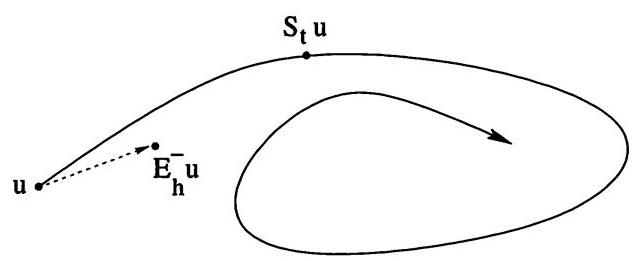
\includegraphics[width=0.6\textwidth]{images/bo_d6ik6nn7aajc739ct1l0_136_739_911_639_261_0.jpg}
\caption{右:依据\eqref{eq:scalar-backward-euler-average}或\eqref{eq:backward-euler-average}，步长为 $h > 0$ 的后向 Euler 逼近是轨迹 $t \mapsto  {S}_{t}u$ 上各点的加权平均，权重呈指数衰减 $w\left( t\right)  = {e}^{-t/h}/h$.}
\label{fig:generator-density}
\end{figure}

\section{预解式}

半群 $\left\{  {{S}_{t};t \geq  0}\right\}$ 与其生成元 $A$ 之间的关键联系由所谓“预解式”给出.该概念借助后向 Euler 逼近最易理解.

假设我们欲用后向Euler逼近近似求解\eqref{eq:evolution-equation}.于是固定时间步长$h > 0$ ，并迭代求解
\[
u\left( {t + h}\right)  = u\left( t\right)  + {hAu}\left( {t + h}\right) .
\]

在每一步中，给定值 $u\left( t\right)  \in  X$ ，我们需计算
\[
u\left( {t + h}\right)  = {\left( I - hA\right) }^{-1}u\left( t\right) .
\]

后向Euler算子
\begin{equation}\tag{7.17}\label{eq:backward-euler-operator}
{E}_{h}^{ - } \doteq  {\left( I - hA\right) }^{-1}
\end{equation}

当 $h > 0$ 较小时，该算子在半群理论中起着关键作用.给定 $A$ ，可通过该算子以两种主要方式恢复Cauchy问题\eqref{eq:evolution-equation}的解.

\subsection{作为后向Euler逼近的极限}

对固定的$\tau  > 0$，考虑时间步长 $h = \tau /n$ .经过 $n$ 步后，后向Euler逼近格式给出
\[
u\left( \tau \right)  \approx  {E}_{\tau /n}^{ - } \circ  \cdots  \circ  {E}_{\tau /n}^{ - } = {\left( I - \frac{\tau }{n}A\right) }^{-n}\bar{u}.
\]

保持 $\tau$ 固定并令 $n \rightarrow  \infty$ ，我们期望在极限下恢复\eqref{eq:evolution-equation}的精确解:
\begin{equation}\tag{7.18}\label{eq:backward-euler-limit}
u\left( \tau \right)  = {S}_{\tau }\bar{u} \doteq  \mathop{\lim }\limits_{{n \rightarrow  \infty }}{\left( I - \frac{\tau }{n}A\right) }^{-n}\bar{u}.
\end{equation}

\subsection{作为近似演化方程解的极限}

再次固定时间步长 $h > 0$ ，并设 $\lambda  = 1/h$ .然后将算子 ${A}_{\lambda } : X \mapsto  X$ 定义为
\[
{A}_{\lambda }u \doteq  A{E}_{h}^{ - }u = A{\left( I - hA\right) }^{-1}u.
\]

换言之， ${A}_{\lambda }u$ 是 $A$ 在 $u$ 处的取值，而非在 ${E}_{h}^{ - }u$ 处，即在后向Euler逼近的第一步中、取 $h = 1/\lambda$ 时的值.事实表明，当 $h > 0$ 足够小时， ${A}_{\lambda } = {A}_{1/h}$ 是一个定义良好且有界的线性算子.因此，我们可以考虑指数型算子 ${e}^{t{A}_{\lambda }} = \mathop{\sum }\limits_{{k \geq  0}}{\left( t{A}_{\lambda }\right) }^{k}/k$ ！并定义
\begin{equation}\tag{7.19}\label{eq:exponential-approx-limit}
u\left( t\right)  = {S}_{t}\bar{u} \doteq  \mathop{\lim }\limits_{{\lambda  \rightarrow  \infty }}{e}^{t{A}_{\lambda }}\bar{u}.
\end{equation}

\begin{instance}\label{ins:scalar-euler}
考虑标量常微分方程
\[
\dot{x} = {ax},\;x\left( 0\right)  = \bar{x}.
\]

其解为 $x\left( t\right)  = {e}^{ta}\bar{x}$ .此时我们平凡地有
\[
{a}_{\lambda } = {a}_{1/h} = \frac{a}{1 - {ha}},\;{e}^{at}\bar{x} = \mathop{\lim }\limits_{{h \rightarrow  0}}{e}^{t{a}_{1/h}}\bar{x} = \mathop{\lim }\limits_{{h \rightarrow  0 + }}{e}^{{ta}/\left( {1 - {ha}}\right) }\bar{x}.
\]

这对应于极限\eqref{eq:exponential-approx-limit}.另一方面，极限\eqref{eq:backward-euler-limit}与恒等式相关
\[
{e}^{\tau a} = \mathop{\lim }\limits_{{n \rightarrow  \infty }}{\left( 1 - \frac{\tau }{n}a\right) }^{-n}
\]

注意，当 $0 < h < {a}^{-1}$ 时，还成立如下恒等式
\begin{equation}\tag{7.20}\label{eq:scalar-backward-euler-average}
{\int }_{0}^{\infty }\frac{{e}^{-t/h}}{h}{\d t} = 1,\;{\left( 1 - ha\right) }^{-1}\bar{x} = {\int }_{0}^{\infty }\left( \frac{{e}^{-t/h}}{h}\right) {e}^{ta}\bar{x}{\d t}.
\end{equation}

第二个恒等式表明，后向Euler算子 ${E}_{h}^{ - }\bar{x} = \; {\left( 1 - ha\right) }^{-1}\bar{x}$ 可通过沿轨迹 $t \mapsto  {e}^{ta}\bar{x}$ 取点并赋予指数衰减权重 $w\left( t\right)  = {h}^{-1}{e}^{-t/h}$ 进行加权平均而得到.
\end{instance}

受前述分析启发，我们引入若干定义.

\begin{definition}[预解集与预解算子]\label{def:resolvent}
设 $A$ 为Banach空间 $X$ 上的线性算子. $A$ 的\colorbf{预解集}是使得算子
\[
{\lambda I} - A : \operatorname{Dom}\left( A\right)  \mapsto  X
\]
是单射且满射的所有实数 $\lambda$ 构成的集合 $\rho \left( A\right)$.\par
若 $\lambda  \in  \rho \left( A\right)$ ，则\colorbf{预解算子}${R}_{\lambda } : X \mapsto  X$ 定义为
\[
{R}_{\lambda }u \doteq  {\left( \lambda I - A\right) }^{-1}u
\]
\end{definition}
我们指出，若 $A$ 是闭算子，则由闭图像定理可知，算子 ${R}_{\lambda } : X \mapsto  \operatorname{Dom}\left( A\right)  \subseteq  X$ 是有界线性算子.此外
\[
A{R}_{\lambda }u = {R}_{\lambda }{Au}\;\text{ if }u \in  \operatorname{Dom}\left( A\right) .
\]

预解式与后向Euler算子之间存在紧密联系.即
\[
\lambda {R}_{\lambda } = {E}_{1/\lambda }^{ - }
\]

\begin{theorem}[预解式恒等式]\label{thm:resolvent-identities}
设 $A$ 为闭线性算子.若 $\lambda ,\mu  \in  \rho \left( A\right)$ ，则
\begin{equation}\tag{7.21}\label{eq:resolvent-identity}
{R}_{\lambda } - {R}_{\mu } = \left( {\mu  - \lambda }\right) {R}_{\lambda }{R}_{\mu }
\end{equation}
\vspace{-2.2 em}
\begin{equation}\tag{7.22}\label{eq:resolvent-commute}
{R}_{\lambda }{R}_{\mu } = {R}_{\mu }{R}_{\lambda }
\end{equation}
\end{theorem}
\begin{proof}
对任意 $u \in  X$ ，有
\[
v \doteq  {R}_{\lambda }u - {R}_{\mu }u = {\left( \lambda I - A\right) }^{-1}u - {\left( \mu I - A\right) }^{-1}u \in  \operatorname{Dom}\left( A\right) ,
\]

$\left( {{\lambda I} - A}\right) v = u - \left( {{\lambda I} - {\mu I} + {\mu I} - A}\right) {\left( \mu I - A\right) }^{-1}u = \left( {\mu  - \lambda }\right) {\left( \mu I - A\right) }^{-1}u.$\par
将算子 ${\left( \lambda I - A\right) }^{-1}$ 作用于上述恒等式两边，即得\eqref{eq:resolvent-identity}.

接下来，利用\eqref{eq:resolvent-identity}，对预解集 $\rho \left( A\right)$ 中的任意 $\lambda  \neq  \mu$ ，可得
\[
{R}_{\lambda }{R}_{\mu } = \frac{{R}_{\lambda } - {R}_{\mu }}{\lambda  - \mu } = \frac{{R}_{\mu } - {R}_{\lambda }}{\mu  - \lambda } = {R}_{\mu }{R}_{\lambda }.
\]
\end{proof}

\begin{theorem}[预解式的积分表达式]\label{thm:resolvent-integral}
设 $\left\{  {{S}_{t};t \geq  0}\right\}$ 是$\omega$类半群，其生成元为 $A$ .则对每个 $\lambda  > \omega$，均有 $\lambda  \in  \rho \left( A\right)$ ，且
\begin{equation}\tag{7.23}\label{eq:resolvent-integral-formula}
{R}_{\lambda }u = {\int }_{0}^{\infty }{e}^{-{t\lambda }}{S}_{t}{u\d t}
\end{equation}

此外，
\begin{equation}\tag{7.24}\label{eq:resolvent-bound}
\norm{R}_{\lambda } \leq  \frac{1}{\lambda  - \omega }
\end{equation}


\end{theorem}
\begin{proof}
1. 由假设，该半群满足估计式 $\norm{S}_{t} \leq  {e}^{t\omega }$ .因此\eqref{eq:resolvent-integral-formula}中的积分绝对收敛:
\begin{equation}\tag{7.25}\label{eq:resolvent-integral-estimate}
\norm{{\int }_{0}^{\infty }{e}^{-{t\lambda }}{S}_{t}{u\d t}} \leq  {\int }_{0}^{\infty }{e}^{t\lambda }\norm{S}_{t}\| u\| {\d t} \leq  {\int }_{0}^{\infty }{e}^{\left( {\omega  - \lambda }\right) t}\| u\| {\d t} \leq  \frac{1}{\lambda  - \omega }\| u\| .
\end{equation}

定义
\[
{\widetilde{R}}_{\lambda }u \doteq  {\int }_{0}^{\infty }{e}^{-{t\lambda }}{S}_{t}{u\d t}
\]

上述估计表明 ${\widetilde{R}}_{\lambda }$ 是有界线性算子，其范数为
\[
\norm{\widetilde{R}}_{\lambda } \leq  \frac{1}{\lambda  - \omega }
\]

\noindent 2. 我们现证
\begin{equation}\tag{7.26}\label{eq:resolvent-surjective}
\left( {{\lambda I} - A}\right) {\widetilde{R}}_{\lambda }u = u\;\forall\,u \in  X.
\end{equation}

事实上，对任意 $h > 0$ ，有
{\begin{align*}
    \frac{{S}_{h}{\widetilde{R}}_{\lambda }u - {\widetilde{R}}_{\lambda }u}{h} &= \frac{1}{h}{\int }_{0}^{\infty }{e}^{-{\lambda t}}\left( {{S}_{t + h}u - {S}_{t}u}\right) {\d t} \\
    &= \frac{1}{h}{\int }_{0}^{\infty }\left( {{e}^{-\lambda \left( {t - h}\right) } - {e}^{-{\lambda t}}}\right) {S}_{t}{u\d t} - \frac{1}{h}{\int }_{0}^{h}{e}^{-\lambda \left( {t - h}\right) }{S}_{t}{u\d t} \\
    &= \left( \frac{{e}^{\lambda h} - 1}{h}\right) {\int }_{0}^{\infty }{e}^{-{\lambda t}}{S}_{t}{u\d t} - \frac{{e}^{\lambda h}}{h}{\int }_{0}^{h}{e}^{-{\lambda t}}{S}_{t}{u\d t}.
\end{align*}}
令 $h \rightarrow  0 +$ 取极限，得
\[
\mathop{\lim }\limits_{{h \rightarrow  0 + }}\frac{{S}_{h}{\widetilde{R}}_{\lambda }u - {\widetilde{R}}_{\lambda }u}{h} = \lambda {\widetilde{R}}_{\lambda }u - u.
\]

由生成元的定义，这意味着
\[
{\widetilde{R}}_{\lambda }u \in  \operatorname{Dom}\left( A\right) ,\;A{\widetilde{R}}_{\lambda }u = \lambda {\widetilde{R}}_{\lambda }u - u,
\]

从而证得\eqref{eq:resolvent-surjective}.

\noindent 3. 恒等式\eqref{eq:resolvent-surjective}已表明映射 $v \mapsto  \left( {{\lambda I} - A}\right) v$ 从 $\operatorname{Dom}\left( A\right)$ 到 $X$ 是满射.我们再证该映射是单射.若 $u \in  \operatorname{Dom}\left( A\right)$ ，则
{\begin{align*}
A{\widetilde{R}}_{\lambda }u &= A{\int }_{0}^{\infty }{e}^{-{\lambda t}}{S}_{t}{u\d t} = {\int }_{0}^{\infty }{e}^{-{\lambda t}}A{S}_{t}{u\d t}\\
&= {\int }_{0}^{\infty }{e}^{-{\lambda t}}{S}_{t}{Au\d t} = {\widetilde{R}}_{\lambda }{Au}
\end{align*}}

这证明了交换关系
\begin{equation}\tag{7.27}\label{eq:resolvent-commutation}
{\widetilde{R}}_{\lambda }\left( {{\lambda I} - A}\right) u = \left( {{\lambda I} - A}\right) {\widetilde{R}}_{\lambda }u\;\forall\,u \in  \operatorname{Dom}\left( A\right) .
\end{equation}

若此时 $\left( {{\lambda I} - A}\right) u = \left( {{\lambda I} - A}\right) v$ ，利用\eqref{eq:resolvent-commutation}式和\eqref{eq:resolvent-surjective}式可得
\[
u = {\widetilde{R}}_{\lambda }\left( {{\lambda I} - A}\right) u = {\widetilde{R}}_{\lambda }\left( {{\lambda I} - A}\right) v = v,
\]

证得映射 $\left( {{\lambda I} - A}\right)$ 是单射.

因此我们得出结论: $\lambda  \in  \rho \left( A\right)$ 且 ${\widetilde{R}}_{\lambda } = {\left( \lambda I - A\right) }^{-1} = {R}_{\lambda }$ .
\end{proof}

\begin{remark}\label{rem:resolvent-laplace}
根据积分表示公式\eqref{eq:resolvent-integral-formula}，预解算子 ${R}_{\lambda }$ 给出了半群 $S$ 的拉普拉斯变换.取 $0 < h = {\lambda }^{-1}$ ，该同一公式表明后向Euler逼近可表示为
\begin{equation}\tag{7.28}\label{eq:backward-euler-average}
{E}_{h}^{ - }u \doteq  {\left( I - hA\right) }^{-1}u = {\int }_{0}^{\infty }\frac{{e}^{-t/h}}{h}{S}_{t}{u\d t}.
\end{equation}

此处积分收敛，前提是 $h$ 足够小:若 $S$ 是$\omega$类半群，则需 $h < {\omega }^{-1}$ .

推广恒等式\eqref{eq:scalar-backward-euler-average}，可见Euler后向逼近的第一步恰与整条轨迹 $t \mapsto  {S}_{t}\bar{u}$ 的加权平均值一致，其指数衰减权重为 $w\left( t\right)  = {h}^{-1}{e}^{-t/h}$ .
\end{remark}

\section{半群的生成}

本节探讨最重要问题:即给定从 $\operatorname{Dom}\left( A\right)  \subset  X$ 到 $X$ 的算子 $A$ ，在何种条件下存在由 $A$ 生成的半群 $\left\{  {{S}_{t};t \geq  0}\right\}$ ？

\begin{theorem}[线性算子生成半群的存在性]\label{thm:hille-yosida}
设 $A$ 是Banach空间 $X$ 上的线性算子，则下列条件等价.
\begin{enumerate}[(i)]
    \item $A$ 是类型为 $\omega$ 的线性算子半群 $\left\{  {{S}_{t};t \geq  0}\right\}$ 的生成元.
    \item A是闭的、稠定算子；此外，每个实数 $\lambda  > \omega$ 均属于 $A$ 的预解集，且
\begin{equation}\tag{7.29}\label{eq:hille-yosida-resolvent-bound}
\norm{\left( \lambda I - A\right) }^{-1} \leq  \frac{1}{\lambda  - \omega },\;\forall\,\lambda  > \omega .
\end{equation}
\end{enumerate}



\end{theorem}
\begin{proof}
(i)$\implies$(ii)已证.因此我们假设(ii)成立，并证明 $A$ 生成$\omega$类半群.证明将分若干步骤完成.

\noindent 1．由假设，对每个 $\lambda  > \omega$ ，预解算子 ${R}_{\lambda } = {\left( \lambda I - A\right) }^{-1}$ 定义良好.于是可考虑如下有界线性算子
\begin{equation}\tag{7.30}\label{eq:Alambda-def}
{A}_{\lambda } \doteq   - {\lambda I} + {\lambda }^{2}{R}_{\lambda } = {\lambda A}{R}_{\lambda }
\end{equation}

注意，令 $h = 1/\lambda$ ，可写为
\[
{A}_{\lambda }u = A{\left( I - hA\right) }^{-1}u = A\left( {{E}_{h}^{ - }u}\right) .
\]

换言之， ${A}_{\lambda }u$ 是 $A$ 在点 ${E}_{h}^{ - }u$ (即从 $u$ 出发、步长为 $h = 1/\lambda$ 的后向Euler步所得之点)处的取值，而非在点 $u$ 处的取值.因此，当 $\lambda$ 充分大(从而 $h = 1/\lambda$ 充分小)时， ${A}_{\lambda }$ 理应是对算子 $A$ 的良好逼近.

\noindent 2. 由于每个 ${A}_{\lambda }$ 均有界，我们可以构造其指数形式为
\[
{e}^{t{A}_{\lambda }} \doteq  \mathop{\sum }\limits_{{k = 0}}^{\infty }\frac{{\left( t{A}_{\lambda }\right) }^{k}}{k!} = {e}^{-{\lambda t}}{e}^{{\lambda }^{2}t{R}_{\lambda }} = {e}^{-{\lambda t}}\mathop{\sum }\limits_{{k = 0}}^{\infty }\frac{{\left( {\lambda }^{2}t\right) }^{k}{R}_{\lambda }^{k}}{k!}.
\]

我们注意到，若 $A$ 无界，则 $\norm{A}_{\lambda } \rightarrow  \infty$ 随 $\lambda  \rightarrow  \infty$ 而变化.然而，对 $t \geq  0$ ，指数算子的范数在 $\lambda  \rightarrow  \infty$ 下保持一致有界.事实上，假设\eqref{eq:hille-yosida-resolvent-bound}连同定义\eqref{eq:Alambda-def}给出
\[
\norm{e}^{t{A}_{\lambda }} \leq  {e}^{-{\lambda t}}\mathop{\sum }\limits_{{k = 0}}^{\infty }\frac{{\left( {\lambda }^{2}t\right) }^{k}{\norm{R}_{\lambda }}^{k}}{k!} \leq  {e}^{-{\lambda t}}{e}^{{\lambda }^{2}t/\left( {\lambda  - \omega }\right) } = {e}^{{\lambda \omega t}/\left( {\lambda  - \omega }\right) }.
\]

特别地，一旦 $\lambda  \geq  {2\omega }$ ，即有
\begin{equation}\tag{7.31}\label{eq:exp-Alambda-bound}
\norm{e}^{t{A}_{\lambda }} \leq  {e}^{2\omega t}\;\forall\,t \geq  0.
\end{equation}

\noindent 3. 在此步骤中，我们建立极限
\begin{equation}\tag{7.32}\label{eq:Alambda-converges-on-domain}
\mathop{\lim }\limits_{{\lambda  \rightarrow  \infty }}{A}_{\lambda }v = {Av}\;\forall\,v \in  \operatorname{Dom}\left( A\right) .
\end{equation}

为证明\eqref{eq:Alambda-converges-on-domain}，我们从恒等式出发
\[
\lambda {R}_{\lambda }u - u = A{R}_{\lambda }u = {R}_{\lambda }{Au}
\]
该式对所有 $u \in  \operatorname{Dom}\left( A\right)$ 均成立.由此可得
\[
\norm{\lambda {R}_{\lambda }u - u}\; = \;\norm{{R}_{\lambda }{Au}}\; \leq  \;\norm{R}_{\lambda }\norm{Au}\; \leq  \;\frac{1}{\lambda  - \omega }\| {Au}\| \; \rightarrow  \;0\;\text{ as }\lambda  \rightarrow  \infty .
\]

因此
\[
\mathop{\lim }\limits_{{\lambda  \rightarrow  \infty }}\lambda {R}_{\lambda }u = u\;\forall\,u \in  \operatorname{Dom}\left( A\right) .
\]

更一般地，利用 $\operatorname{Dom}\left( A\right)$ 在 $X$ 中稠密这一事实，可以证明上述极限对所有 $u \in  X$成立.事实上，对任意 $u \in  X$ 和 $\varepsilon  > 0$ ，存在 $v \in  \operatorname{Dom}\left( A\right)$ 使得 $\| u - v\|  < \varepsilon$ .应用三角不等式，得到
{\setjot[-2]\begin{align*}
    &\quad\limsup_{{\lambda  \rightarrow  \infty }}\norm{\lambda {R}_{\lambda }u - u} \\
    &\leq  \limsup_{{\lambda  \rightarrow  \infty }}\norm{\lambda {R}_{\lambda }u - \lambda {R}_{\lambda }v} + \limsup_{{\lambda  \rightarrow  \infty }}\norm{\lambda {R}_{\lambda }v - v} + \| v - u\| \\
    &\leq  \limsup_{{\lambda  \rightarrow  \infty }}\norm{\lambda {R}_{\lambda }}\| u - v\|  + 0 + \| v - u\|\\
    &\leq  \limsup_{{\lambda  \rightarrow  \infty }}\frac{\lambda }{\lambda  - \omega }\varepsilon  + \varepsilon  = {2\varepsilon }
\end{align*}}

由于 $\varepsilon  > 0$ 是任意的，这证明了
\begin{equation}\tag{7.33}\label{eq:lambdaRlambda-to-I}
\mathop{\lim }\limits_{{\lambda  \rightarrow  \infty }}\lambda {R}_{\lambda }u = u\;\forall\,u \in  X.
\end{equation}

对于时间步长为 $h = 1/\lambda$ 的后向Euler逼近，由\eqref{eq:lambdaRlambda-to-I}可得
\[
\mathop{\lim }\limits_{{h \rightarrow  0 + }}{E}_{h}^{ - }u = u\;\forall\,u \in  X.
\]

若 $v \in  \operatorname{Dom}\left( A\right)$ ，则在\eqref{eq:lambdaRlambda-to-I}中可取 $u = {Av}$ ，并得出
\[
\mathop{\lim }\limits_{{\lambda  \rightarrow  \infty }}{A}_{\lambda }v = \mathop{\lim }\limits_{{\lambda  \rightarrow  \infty }}{\lambda A}{R}_{\lambda }v = \mathop{\lim }\limits_{{\lambda  \rightarrow  \infty }}\lambda {R}_{\lambda }{Av} = \mathop{\lim }\limits_{{\lambda  \rightarrow  \infty }}\lambda {R}_{\lambda }u = u = {Av}.
\]

这证明了\eqref{eq:Alambda-converges-on-domain}.

\noindent 4. 固定任意 $t \geq  0$ .我们声称:当 $\lambda  \rightarrow  \infty$ 时，一族一致有界算子 ${e}^{t{A}_{\lambda }}$ 收敛于某个线性算子，记为 ${S}_{t}$ .

为证明这一点，对 $\lambda ,\mu  > {2\omega }$ ，我们将估计差值 ${e}^{t{A}_{\lambda }} - {e}^{t{A}_{\mu }}$ .

交换关系 ${R}_{\lambda }{R}_{\mu } = {R}_{\mu }{R}_{\lambda }$ 蕴含 ${A}_{\lambda }{A}_{\mu } = {A}_{\mu }{A}_{\lambda }$ .因此
\[
{A}_{\mu }{e}^{t{A}_{\lambda }} = {A}_{\mu }\mathop{\sum }\limits_{{k = 0}}^{\infty }\frac{{\left( t{A}_{\lambda }\right) }^{k}}{k!} = {e}^{t{A}_{\lambda }}{A}_{\mu }.
\]

于是对每个 $u \in  X$ ，均有
{\begin{align*}
{e}^{t{A}_{\lambda }}u - {e}^{t{A}_{\mu }}u &= {\int }_{0}^{t}\frac{d}{\d s}\left(  {{e}^{\left( {t - s}\right) {A}_{\mu }}{e}^{s{A}_{\lambda }}u}\right)  {\d s}\\
&= {\int }_{0}^{t}{e}^{\left( {t - s}\right) {A}_{\mu }}\left( {{A}_{\lambda } - {A}_{\mu }}\right) {e}^{s{A}_{\lambda }}{u\d s} = {\int }_{0}^{t}{e}^{\left( {t - s}\right) {A}_{\mu }}{e}^{s{A}_{\lambda }}\left( {{A}_{\lambda }u - {A}_{\mu }u}\right) {\d s}.
\end{align*}}

由\eqref{eq:exp-Alambda-bound}式可知
\[
\norm{{e}^{t{A}_{\lambda }}u - {e}^{t{A}_{\mu }}u}\; \leq  \;{\int }_{0}^{t}{e}^{2\left( {t - s}\right) \omega }{e}^{2s\omega }\norm{{A}_{\lambda }u - {A}_{\mu }u}{\d s}\; = \;t\;{e}^{2\omega t}\norm{{A}_{\lambda }u - {A}_{\mu }u}.
\]

若 $u \in  \operatorname{Dom}\left( A\right)$ ，则\eqref{eq:Alambda-converges-on-domain}式给出 ${A}_{\lambda }u \rightarrow  {Au}$ 与 ${A}_{\mu }u \rightarrow  {Au}$ 为 $\lambda ,\mu  \rightarrow  \infty$ .因此
\[
\limsup_{{\lambda ,\mu  \rightarrow  \infty }}\norm{{e}^{t{A}_{\lambda }}u - {e}^{t{A}_{\mu }}u} \leq  t{e}^{2\omega t}\limsup_{{\lambda ,\mu  \rightarrow  \infty }}\norm{{A}_{\lambda }u - {A}_{\mu }u} = 0.
\]\par

\begin{figure}[H]
\centering
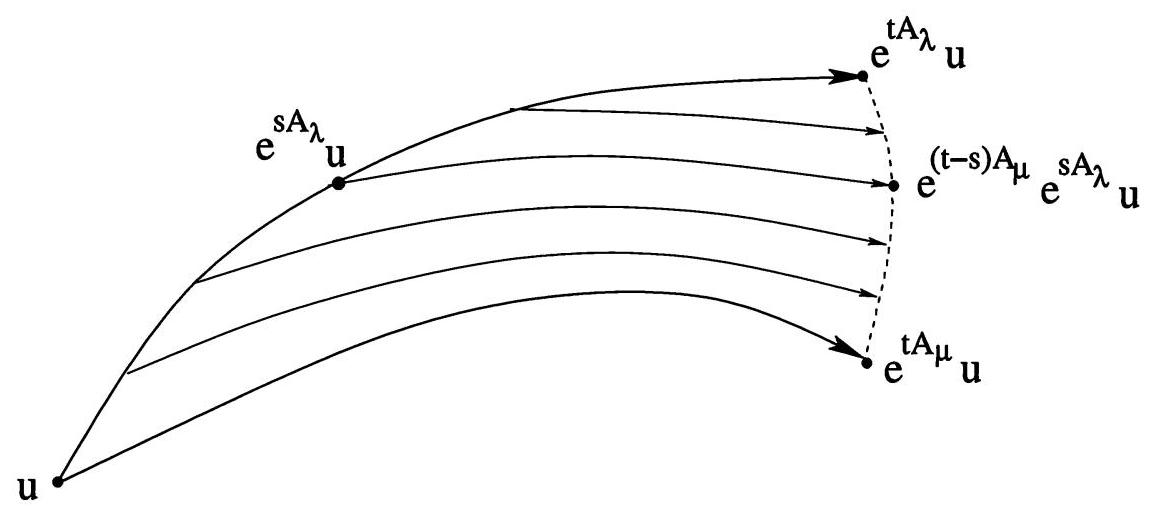
\includegraphics[width=0.75\textwidth]{images/bo_d6ik6nn7aajc739ct1l0_143_164_1407_1153_511_0.jpg}
\captionof{figure}{证明逼近序列 ${e}^{t{A}_{\lambda }}$ 当 $\lambda  \rightarrow  \infty$ 时的收敛性.差值 $\norm{{e}^{t{A}_{\lambda }}u - {e}^{t{A}_{\mu }}u}$ 可通过曲线 $s \mapsto  {e}^{\left( {t - s}\right) {A}_{\mu }}{e}^{s{A}_{\lambda }}u$ 的长度估计，其中 $s \in  \left(  {0,t}\right)$ .}
\label{fig:Alambda-convergence}
\end{figure}

利用三角不等式，我们进一步证明:对任意 $v \in  X$ ，该极限在 $t$ 取遍有界区间时一致成立.

事实上，给定 $\varepsilon  > 0$ ，选取满足 $\| u - v\|  \leq  \varepsilon$ 的 $u \in  \operatorname{Dom}\left( A\right)$ .则
{\setjot[-2]\begin{align*}
    &\quad\limsup_{{\lambda ,\mu  \rightarrow  \infty }}\norm{{e}^{t{A}_{\lambda }}v - {e}^{t{A}_{\mu }}v}\\
    &\leq  \limsup_{{\lambda  \rightarrow  \infty }}\norm{{e}^{t{A}_{\lambda }}v - {e}^{t{A}_{\lambda }}u} + \limsup_{{\lambda ,\mu  \rightarrow  \infty }}\norm{{e}^{t{A}_{\lambda }}u - {e}^{t{A}_{\mu }}u}\\
    &\quad+\limsup_{{\mu  \rightarrow  \infty }}\norm{{e}^{t{A}_{\mu }}u - {e}^{t{A}_{\mu }}v}\\
    &\leq  2\limsup_{{\lambda  \rightarrow  \infty }}\norm{e}^{t{A}_{\lambda }}\norm{v - u} \leq  2{e}^{2\omega t}\varepsilon
\end{align*}}

由于 $\varepsilon  > 0$ 是任意的，故所断言成立.

\noindent 5．由前一步可知，对任意 $t \geq  0$ 与 $u \in  X$ ，下列极限良定义:
\[
{S}_{t}u \doteq  \mathop{\lim }\limits_{{\lambda  \rightarrow  \infty }}{e}^{t{A}_{\lambda }}u
\]

我们断言 $\left\{  {{S}_{t};t \geq  0}\right\}$ 是类型为 $\omega$ 的强连续半群.

事实上，半群性质由下式推出
\[
{S}_{t}{S}_{s}u = \mathop{\lim }\limits_{{\lambda  \rightarrow  \infty }}{e}^{t{A}_{\lambda }}{e}^{s{A}_{\lambda }}u = \mathop{\lim }\limits_{{\lambda  \rightarrow  \infty }}{e}^{\left( {t + s}\right) {A}_{\lambda }}u = {S}_{t + s}u.
\]

对固定 $u \in  X$ ，映射 $t \mapsto  {S}_{t}u$ 连续，因其为连续映射 $t \mapsto  {e}^{t{A}_{\lambda }}u$ 在 $t$ 取遍有界区间时的一致极限.

最后，对任意满足 $\| u\|  \leq  1$ 的 $t \geq  0$ 与 $u \in  X$ ，我们有如下估计
{\setjot[-2]\begin{align*}
\norm{{S}_{t}u} &= \mathop{\lim }\limits_{{\lambda  \rightarrow  \infty }}\norm{{e}^{t{A}_{\lambda }}u} \leq  \limsup_{{\lambda  \rightarrow  \infty }}\norm{e}^{t{A}_{\lambda }}\| u\|\\
&\leq  \mathop{\lim }\limits_{{\lambda  \rightarrow  \infty }}{e}^{{t\lambda \omega }/\left( {\lambda  - \omega }\right) }\| u\|  = {e}^{t\omega }\| u\| .
\end{align*}}

这证明了 $\norm{S}_{t} \leq  {e}^{t\omega }$ ，即该半群为类型 $\omega$ .

\noindent 6．尚需证明线性算子 $A$ 确为该半群的生成元.为此，记 $B$ 为半群 $\left\{  {{S}_{t};t \geq  0}\right\}$ 的生成元.据前述分析，已知 $B$ 是定义在 $\operatorname{Dom}\left( B\right)$ (在 $X$ 中稠密)上的线性闭算子.需证 $B = A$ .

由于 ${A}_{\lambda }$ 是半群 $\left\{  {{e}^{t{A}_{\lambda }};t \geq  0}\right\}$ 的生成元，故对任意 $\lambda  > \omega$ ，有
\begin{equation}\tag{7.34}\label{eq:exp-Alambda-difference}
{e}^{t{A}_{\lambda }}u - u = {\int }_{0}^{t}{e}^{s{A}_{\lambda }}{A}_{\lambda }{u\d s}.
\end{equation}

此外，对 $u \in  \operatorname{Dom}\left( A\right)$ ，三角不等式给出
\begin{equation}\tag{7.35}\label{eq:Alambda-estimate}
\norm{{e}^{s{A}_{\lambda }}{A}_{\lambda }u - {S}_{s}{Au}}  \leq   \norm{e}^{s{A}_{\lambda }}\norm{{A}_{\lambda }u - {Au}} + \norm{{e}^{s{A}_{\lambda }}{Au} - {S}_{s}{Au}}.
\end{equation}

当 $\lambda  \rightarrow  \infty$ 时，\eqref{eq:Alambda-estimate}式右端趋于零，且在 $s$ 取遍有界区间时一致成立.于\eqref{eq:exp-Alambda-difference}式中令 $\lambda  \rightarrow  \infty$ 取极限，即得
\begin{equation}\tag{7.36}\label{eq:semigroup-variation-of-constants-linear}
{S}_{t}u - u = {\int }_{0}^{t}{S}_{s}{Au\d s}\;\forall\,t \geq  0,u \in  \operatorname{Dom}\left( A\right) .
\end{equation}

因此， $\operatorname{Dom}\left( B\right)  \supseteq  \operatorname{Dom}\left( A\right)$ 且
\[
{Bu} = \mathop{\lim }\limits_{{h \rightarrow  0 + }}\frac{{S}_{t}u - u}{t} = \mathop{\lim }\limits_{{t \rightarrow  0 + }}\frac{1}{t}{\int }_{0}^{t}{S}_{s}{Au\d s} = {Au}\;\forall\,u \in  \operatorname{Dom}\left( A\right) .
\]

为证 $A = B$ ，尚需证明 $\operatorname{Dom}\left( B\right)  \subseteq  \operatorname{Dom}\left( A\right)$ .为此，任取 $\lambda  > \omega$ .已知算子
\[
{\lambda I} - A : \operatorname{Dom}\left( A\right)  \mapsto  X\;\text{ and }\;{\lambda I} - B : \operatorname{Dom}\left( B\right)  \mapsto  X
\]
均为单射且满射.特别地， ${\lambda I} - B$ 在 $\operatorname{Dom}\left( A\right)$ 上的限制与 ${\lambda I} - A$ 重合，故为满射.因此，该算子 ${\lambda I} - B$ 无法在保持单射性的前提下延拓至严格大于 $\operatorname{Dom}\left( A\right)$ 的定义域.这表明 $\operatorname{Dom}\left( B\right)  = \operatorname{Dom}\left( A\right)$ ，证毕.
\end{proof}

现考察唯一性.给定一族线性算子半群 $\left\{  {{S}_{t};t \geq  0}\right\}$ ，其生成元由\eqref{eq:generator-def}式中的极限唯一确定.反之，若给定满足定理\ref{thm:hille-yosida}中条件(ii)的线性算子 $A$ ，则我们证明:由 $A$ 生成的半群被唯一确定.

\begin{theorem}[半群的唯一性]\label{thm:semigroup-uniqueness}
设 $\left\{  {S}_{t}\right\}  ,\left\{  {\widetilde{S}}_{t}\right\}$ 为两个强连续线性算子半群，且具有相同的生成元 $A$ .则对每个 $t \geq  0$，均有 ${S}_{t} = {\widetilde{S}}_{t}$ .
\end{theorem}

\begin{proof}
令 $u \in  \operatorname{Dom}\left( A\right)$ .则对每个 $0 \leq  s \leq  t$ ，有 ${\widetilde{S}}_{s}u \in  \operatorname{Dom}\left( A\right)$ 且 ${S}_{t - s}{\widetilde{S}}_{s}u \in  \operatorname{Dom}\left( A\right)$.于是可估计
\[
{\widetilde{S}}_{t}u - {S}_{t}u = {\int }_{0}^{t}\frac{d}{\d s}\left(  {{S}_{t - s}{\widetilde{S}}_{s}u}\right)  {\d s} = {\int }_{0}^{t}\left(  {{S}_{t - s}A{\widetilde{S}}_{s}u - A{S}_{t - s}{\widetilde{S}}_{s}u}\right)  {\d s} = 0.
\]

事实上，
{\setjot[-1]\begin{align*}
    \frac{\d}{\d s}\left(  {{S}_{t - s}{\widetilde{S}}_{s}u}\right)   &= \mathop{\lim }\limits_{{h \rightarrow  0}}\frac{{S}_{t - s - h}\left( {{\widetilde{S}}_{s + h}u}\right)  - {S}_{t - s}{\widetilde{S}}_{s}u}{h}\\
    &= \mathop{\lim }\limits_{{h \rightarrow  0}}\frac{{S}_{t - s - h}\left( {{\widetilde{S}}_{s + h}u - {\widetilde{S}}_{s}u}\right) }{h} + \mathop{\lim }\limits_{{h \rightarrow  0}}\frac{{S}_{t - s - h}\left( {{\widetilde{S}}_{s}u}\right)  - {S}_{t - s}\left( {{\widetilde{S}}_{s}u}\right) }{h}\\
    &= {S}_{t - s}\left( {A{\widetilde{S}}_{s}u}\right)  - A{S}_{t - s}\left( {{\widetilde{S}}_{s}u}\right)  = 0.
\end{align*}}


这表明:对每个固定的 $t \geq  0$ ，有界线性算子 ${S}_{t}$ 与 ${\widetilde{S}}_{t}$ 在稠密子集 $\operatorname{Dom}\left( A\right)$ 上重合.故 ${S}_{t} = {\widetilde{S}}_{t}$ .
\end{proof}

半群理论在演化型偏微分方程求解中的应用将在第9章予以说明.

\section{习题}

\begin{rbhw}[index=1]
假设\eqref{eq:diagonal-operator-l1}式中的算子 $A$ 是扇形的，即对某个 $\omega  \in  \mathbb{R}$ 和某个角 $\overline{\theta } < \pi /2$ ，\eqref{eq:sectorial-eigs}式成立.

(i) 对 $t > 0$ ，给出算子 $\norm{A{e}^{tA}}$ 范数的先验估计，该估计仅依赖于 $\omega ,\overline{\theta }$ .

(ii) 更一般地，对 $t > 0$ 和 $k \geq  1$ ，证明算子 ${A}^{k}{e}^{tA}$ 同样有界，并估计范数 $\norm{{A}^{k}{e}^{tA}}$ .

\end{rbhw}

\begin{rbhw}
设 $A$ 是一个压缩半群的生成元.证明:对每个 $\lambda  > 0$ ，\eqref{eq:Alambda-def}式中的有界线性算子 ${A}_{\lambda }$ 也生成一个压缩半群.

\end{rbhw}

\begin{rbhw}
固定 $\lambda  > 0$ ，并考虑权函数
\[
w\left( t\right)  = \begin{cases} \lambda {e}^{-{\lambda t}} & \text{ if }t \geq  0, \\  0 & \text{ if }t < 0. \end{cases}
\]

对 $n \geq  1$ 归纳，验证 $n$ 重卷积 ${w}_{n} \doteq  w * w * \cdots  * w$ 由下式给出

\begin{equation}\tag{7.37}\label{eq:wn-convolution}
{w}_{n}\left( t\right)  = \begin{cases} \frac{{\lambda }^{n}}{\left( {n - 1}\right) !}{t}^{n - 1}{e}^{-{\lambda t}} & \text{ if }t \geq  0, \\  0 & \text{ if }t < 0. \end{cases}
\end{equation}

证明 $w\left( \cdot \right)$ 是一个概率测度的密度函数，满足
\[
\text{期望} = {\int }_{0}^{\infty }{tw}\left( t\right) {\d t} = \frac{1}{\lambda }
\]
\[
\text{方差} = {\int }_{0}^{\infty }{\left( t - \frac{1}{\lambda }\right) }^{2}w\left( t\right) {\d t} = {\int }_{0}^{\infty }\left( {{t}^{2} - \frac{1}{{\lambda }^{2}}}\right) w\left( t\right) {\d t} = \frac{1}{{\lambda }^{2}}\text{ . }
\]

因此， ${w}_{n}\left( \cdot \right)$ 是一个均值为 $n/\lambda$ 、方差为 $n/{\lambda }^{2}$ 的概率测度的密度函数.

现固定 $T > 0$ ，并令 ${\lambda }_{n} \doteq  n/T$ .对每个 $n \geq  1$ ，定义
\begin{equation}\tag{7.38}\label{eq:Wn-def}
{W}_{n}\left( t\right)  = \left\{  \begin{aligned} \frac{{\left( n/T\right) }^{n}}{\left( {n - 1}\right) !}{t}^{n - 1}{e}^{-\left( {n/T}\right) t} & & \text{ if }t \geq  0, \\  0 & & \text{ if }t < 0. \end{aligned}\right.
\end{equation}

证明图\ref{fig:Wn-weights}中绘制的 ${W}_{n}\left( \cdot \right)$ 是一个均值为 $n/{\lambda }_{n} = T$ 、方差为 $n/{\left( n/T\right) }^{2} = {T}^{2}/n$ 的概率测度的密度函数.特别地，对每个 $\varepsilon  > 0$ ，有
\begin{equation}\tag{7.39}\label{eq:Wn-concentration}
\mathop{\lim }\limits_{{n \rightarrow  \infty }}\left(  {{\int }_{0}^{T - \varepsilon }{W}_{n}\left( t\right) {\d t} + {\int }_{T + \varepsilon }^{\infty }{W}_{n}\left( t\right) {\d t}}\right)   = 0,\;\mathop{\lim }\limits_{{n \rightarrow  \infty }}{\int }_{T - \varepsilon }^{T + \varepsilon }{W}_{n}\left( t\right) {\d t} = 1.
\end{equation}

\begin{figure}[htbp]
\centering
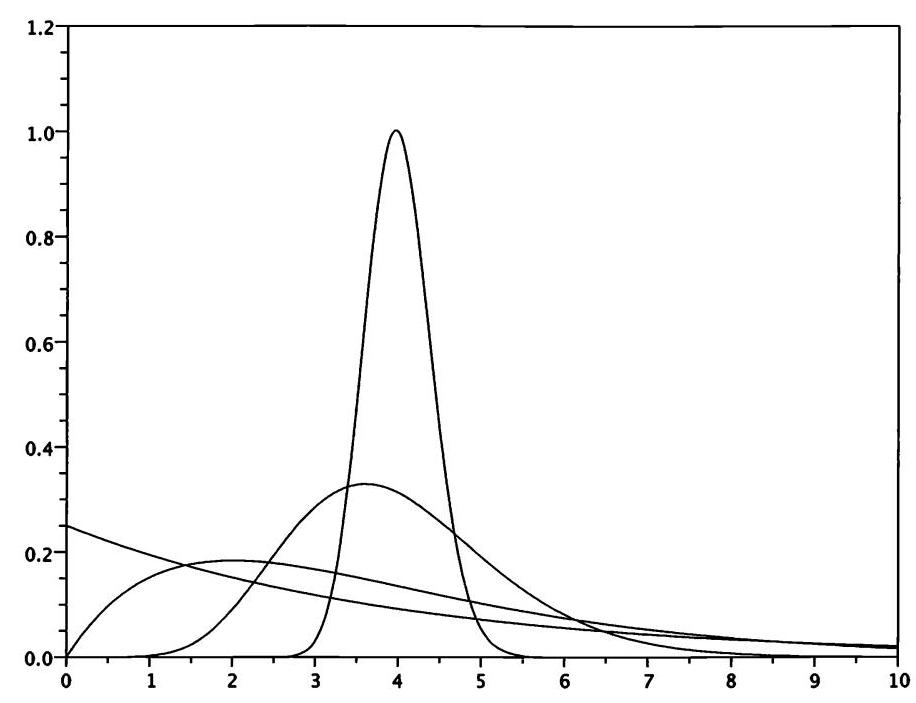
\includegraphics[width=0.8\textwidth]{images/bo_d6ik6nn7aajc739ct1l0_147_261_663_916_703_0.jpg}
\captionof{figure}{由式\eqref{eq:Wn-def}定义的权函数 ${W}_{n}$ 的图像.此处 $T = 4$ ，而 $n = 1,2,{10},{100}$ .所有这些概率分布的平均值均为4，而其方差 $\left( { = {16}/n}\right)$ 随 $n \rightarrow  \infty$ 趋于零.}
\label{fig:Wn-weights}
\end{figure}

\end{rbhw}

\begin{rbhw}
(向后Euler逼近的收敛性)设 $\left\{  {{S}_{t};t \geq  0}\right\}$ 是Banach空间 $X$ 上的一个压缩半群，由线性算子 $A$ 生成.固定 $h > 0$ ，并令 $\lambda  = 1/h$ .对 $n \geq  1$ 进行归纳，将向后Euler逼近公式\eqref{eq:backward-euler-average}推广.即证明
\[
{\left( I - hA\right) }^{-n}u = {\int }_{0}^{\infty }{w}_{n}\left( t\right) {S}_{t}{u\d t}\;\forall\,u \in  X,
\]

其中 ${w}_{n}$ 是式\eqref{eq:wn-convolution}中定义的权函数.

令 $h = T/n$ ，从而 ${\lambda }_{n} = n/T$ .利用\eqref{eq:Wn-concentration}证明:对每个 $u \in  X$ ，有如下收敛性
\[
{\left( I - \frac{T}{n}A\right) }^{-n}u = {\int }_{0}^{\infty }{W}_{n}\left( t\right) {S}_{t}{u\d t} \rightarrow  {S}_{T}u\;\text{ as }n \rightarrow  \infty .
\]

\end{rbhw}

\begin{rbhw}
(正不变集)设 $A$ 是Banach空间 $X$ 上压缩半群 $\left\{  {{S}_{t};t \geq  0}\right\}$ 的生成元.设 $\Omega  \subset  X$ 是一个闭凸子集.证明下列命题等价.

(i) $\Omega$ 是正不变的:若 $u \in  \Omega$ ，则对所有 $t \geq  0$ ，有 ${S}_{t}u \in  \Omega$ .

(ii) $\Omega$ 关于向后Euler算子是不变的:若 $u \in  \Omega$ ，则对每个 $h > 0$ ，均有 ${\left( I - hA\right) }^{-1}u \in  \Omega$ .

\end{rbhw}

\begin{rbhw}
设 $\left\{  {{S}_{t};t \geq  0}\right\}$ 是$\omega$类半群，其生成元为 $A$ .证明:对每个 $\gamma  \in  \mathbb{R}$ ，有界线性算子族 $\left\{  {{e}^{\gamma t}{S}_{t};t \geq  0}\right\}$ 构成一个类型为 $\omega  + \gamma$ 的半群，其生成元为 $A + {\gamma I}$ .

\end{rbhw}

\begin{rbhw}
在空间 ${L}^{p}\left( \mathbb{R}\right)$ 上，考虑由下式定义的线性算子 ${S}_{t}$
\[
\left( {{S}_{t}f}\right) \left( x\right)  = {e}^{-{2t}}f\left( {x + t}\right) .
\]

(i) 证明:线性算子族 $\left\{  {{S}_{t};t \geq  0}\right\}$ 对所有 $1 \leq  p < \infty$ 均构成 ${L}^{p}\left( \mathbb{R}\right)$ 上强连续、压缩的半群.求出该半群的生成元 $A$ . $\operatorname{Dom}\left( A\right)$ 是什么？

(ii) 证明算子族 $\left\{  {{S}_{t};t \geq  0}\right\}$ 在 ${L}^{\infty }\left( \mathbb{R}\right)$ 上 NOT 构成强连续半群.

\end{rbhw}

\begin{rbhw}
设 $\left\{  {{S}_{t};t \geq  0}\right\}$ 是 ${\mathbb{R}}^{n}$ 上的强连续线性算子半群.证明存在一个 $n \times  n$ 矩阵 $A$ ，使得对每个 $t \geq  0$ ，均有 ${S}_{t} = {e}^{tA}$ .

\end{rbhw}

\begin{rbhw}
(半线性方程)设 $A$ 是Banach空间 $X$ 上的线性算子，生成压缩半群 $\left\{  {{S}_{t};t \geq  0}\right\}$.称映射 $u : \left(  {0,T}\right)   \mapsto  X$ 为半线性Cauchy问题的温和解
\begin{equation}\tag{7.40}\label{eq:semilinear-cauchy-problem}
\frac{d}{\d t}u\left( t\right)  = {Au}\left( t\right)  + f\left( {t,u\left( t\right) }\right) ,\;u\left( 0\right)  = \bar{u}
\end{equation}
如果
\begin{equation}\tag{7.41}\label{eq:mild-solution}
u\left( t\right)  = {S}_{t}\bar{u} + {\int }_{0}^{t}{S}_{t - s}f\left( {s,u\left( s\right) }\right) {\d s}\;\forall\,t \in  \left(  {0,T}\right)  .
\end{equation}

(i) 假设 $f : \left(  {0,T}\right)   \times  X \mapsto  X$ 连续且满足如下估计式
\[
\| f\left( {t,x}\right) \|  \leq  M,\;\| f\left( {t,x}\right)  - f\left( {t,y}\right) \|  \leq  L\| x - y\| \;\forall\,t,x,y,
\]

证明Cauchy问题\eqref{eq:semilinear-cauchy-problem}存在唯一温和解.

(ii) 在 $A$ 为有界算子的特殊情形下，即 ${S}_{t} = {e}^{tA}$ 成立，证明 $u\left( \cdot \right)$ 满足\eqref{eq:mild-solution}当且仅当 $u$ 是Cauchy问题\eqref{eq:semilinear-cauchy-problem}的连续可微解.

\end{rbhw}

\begin{rbhw}
固定时间 $T > 0$ .在空间 $X = {L}^{1}\left( \left(  {0,1}\right)  \right)$ 上，构造一个强连续的压缩线性算子半群 $\left\{  {{S}_{t};t \geq  0}\right\}$ ，使得对 $0 \leq  t < T$ 有 $\norm{S}_{t} = 1$ ，但对 $t \geq  T$ 有 $\norm{S}_{t} = 0$ .

\end{rbhw}

\begin{rbhw}
设 $\left\{  {{S}_{t};t \geq  0}\right\}$ 是Banach空间 $X$ 上的强连续压缩线性算子半群.假设对给定时间 $\tau  > 0$ ，算子 ${S}_{\tau }$ 是紧的.证明:对任意 $t > \tau$ ，算子 ${S}_{t}$ 也是紧的.构造一个反例，说明当 $0 \leq \; t < \tau$ 时，算子 ${S}_{t}$ 未必是紧的.

\end{rbhw}

\begin{rbhw}
在空间 ${L}^{1}\left( \mathbb{R}\right)$ 上，考虑定义域为 ${Au} = \frac{\partial }{\partial x}u$ 的算子

$\operatorname{Dom}\left( A\right)  = \left\{  {u \in  {L}^{1}\left( \mathbb{R}\right) ;u\text{ is absolutely continuous, }{u}_{x} \in  {L}^{1}\left( \mathbb{R}\right) }\right\}$ .

(i) 描述由 $A$ 生成的半群 $\left\{  {{S}_{t};t \geq  0}\right\}$ .

(ii) 对任意 $u \in  {L}^{1}\left( \mathbb{R}\right)$ 与 $h > 0$ ，构造后向Euler逼近 ${E}_{h}^{ - }u$ .

(iii) 设 $u \in  {\mathcal{C}}_{c}^{\infty }\left( \mathbb{R}\right)$ 是具有紧支集的光滑函数，例如满足当 $x \notin  \left(  {a,b}\right)$ 时 $u\left( x\right)  = 0$ .对任意时间步长 $h > 0$ ，证明前向Euler逼近 ${\left( {E}_{h}^{ + }\right) }^{n}u = {\left( I + hA\right) }^{n}u$ 良定义，且其支集包含于 $\left(  {a,b}\right)$ .

(iv) 利用(iii)，证明:对每个足够大的时间 $\tau  > 0$ ，函数 ${\left( I + \frac{\tau }{n}A\right) }^{n}u$ 不能随 $n \rightarrow  \infty$ 趋于 ${S}_{\tau }u$ .

\end{rbhw}
